\documentclass[10pt]{article}
\usepackage[utf8]{inputenc}
\usepackage[T1]{fontenc}
\usepackage{amsmath}
\usepackage{amsfonts}
\usepackage{amssymb}
\usepackage[version=4]{mhchem}
\usepackage{stmaryrd}
\usepackage{bbold}
\usepackage{graphicx}
\usepackage[export]{adjustbox}
\graphicspath{ {./images/} }
\usepackage{hyperref}
\hypersetup{colorlinks=true, linkcolor=blue, filecolor=magenta, urlcolor=cyan,}
\urlstyle{same}

\title{Unsupervised Learning }

\author{}
\date{}


\begin{document}
\maketitle
Machine Learning Course - CS-433

Nov 22, 2023

Martin Jaggi

Last updated on: November 20, 2023

credits to Mohammad Emtiyaz Khan \& Rüdiger Urbanke

EPFL

\section*{Unsupervised learning}
How can systems learn when there are no labels available? How to learn a meaningful internal representation for data examples? I.e., to represent them in a way that reflects the semantic structure of the overall collection of input patterns? This question is the central focus of unsupervised learning.

In unsupervised learning, our data consists only of features (or inputs) $\mathbf{x}_{1}, \mathbf{x}_{2}, \ldots, \mathbf{x}_{N}$, vectors in $\mathbb{R}^{D}$, and there are no outputs $y_{n}$ available.

Unsupervised learning seems to play an important role in how living beings learn. Variants of it seem to be more common in the brain than supervised learning.

Two main directions in unsupervised learning are

\begin{itemize}
  \item representation learning and
  \item density estimation \& generative models
\end{itemize}

\section*{Examples}
\section*{Examples for Representation Learning}
Given ratings of movies and viewers, we use matrix factorization to extract useful features (see e.g. Netflix Prize).

\begin{center}
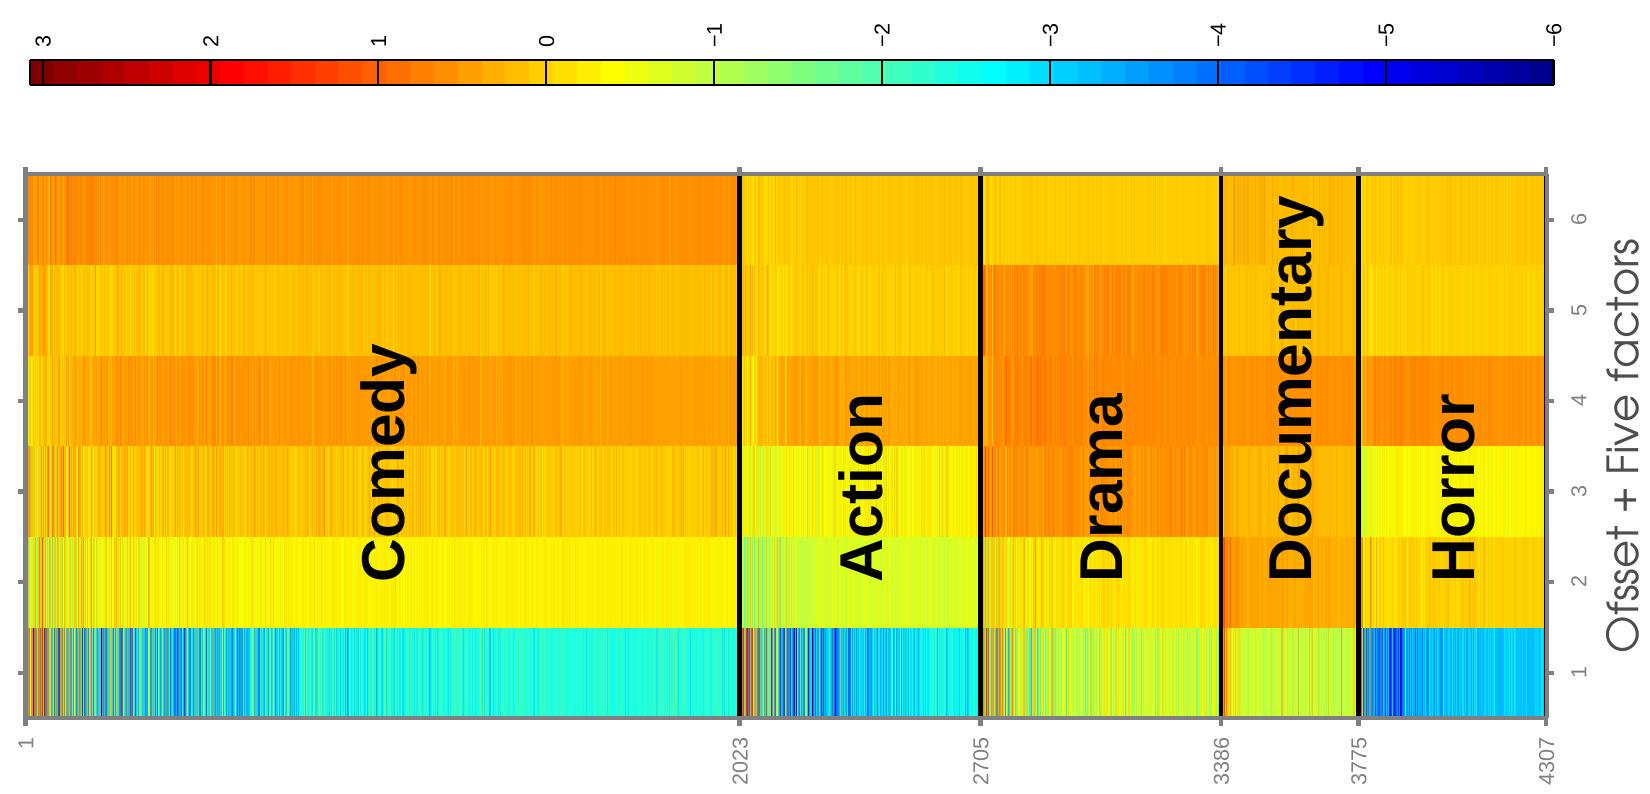
\includegraphics[max width=\textwidth]{2024_01_08_e090cb7d953bac87fc33g-03(3)}
\end{center}


Learning word-representations using matrix-factorizations, word2vec (Mikolov et al. 2013).

\begin{center}
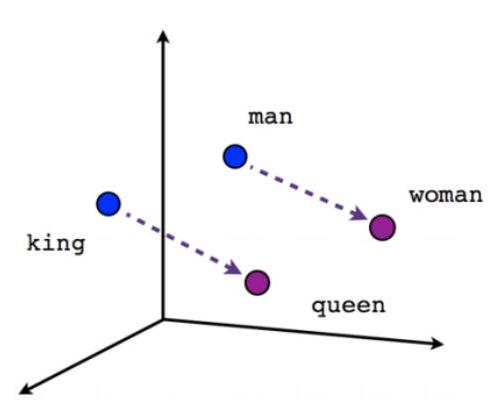
\includegraphics[max width=\textwidth]{2024_01_08_e090cb7d953bac87fc33g-03(2)}
\end{center}

Male-Female

\begin{center}
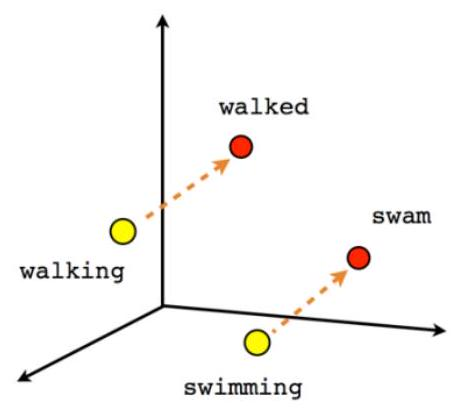
\includegraphics[max width=\textwidth]{2024_01_08_e090cb7d953bac87fc33g-03(1)}
\end{center}

Verb tense

\begin{center}
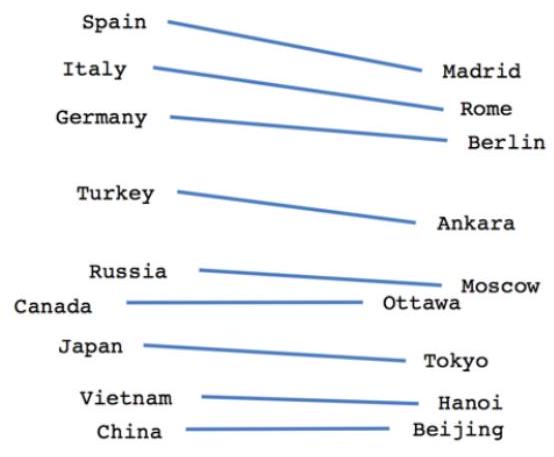
\includegraphics[max width=\textwidth]{2024_01_08_e090cb7d953bac87fc33g-03}
\end{center}

Country-Capital

\section*{Given voting patterns of regions across Switzerland, we use PCA to extract useful features (Etter et al. 2014).}
\begin{center}
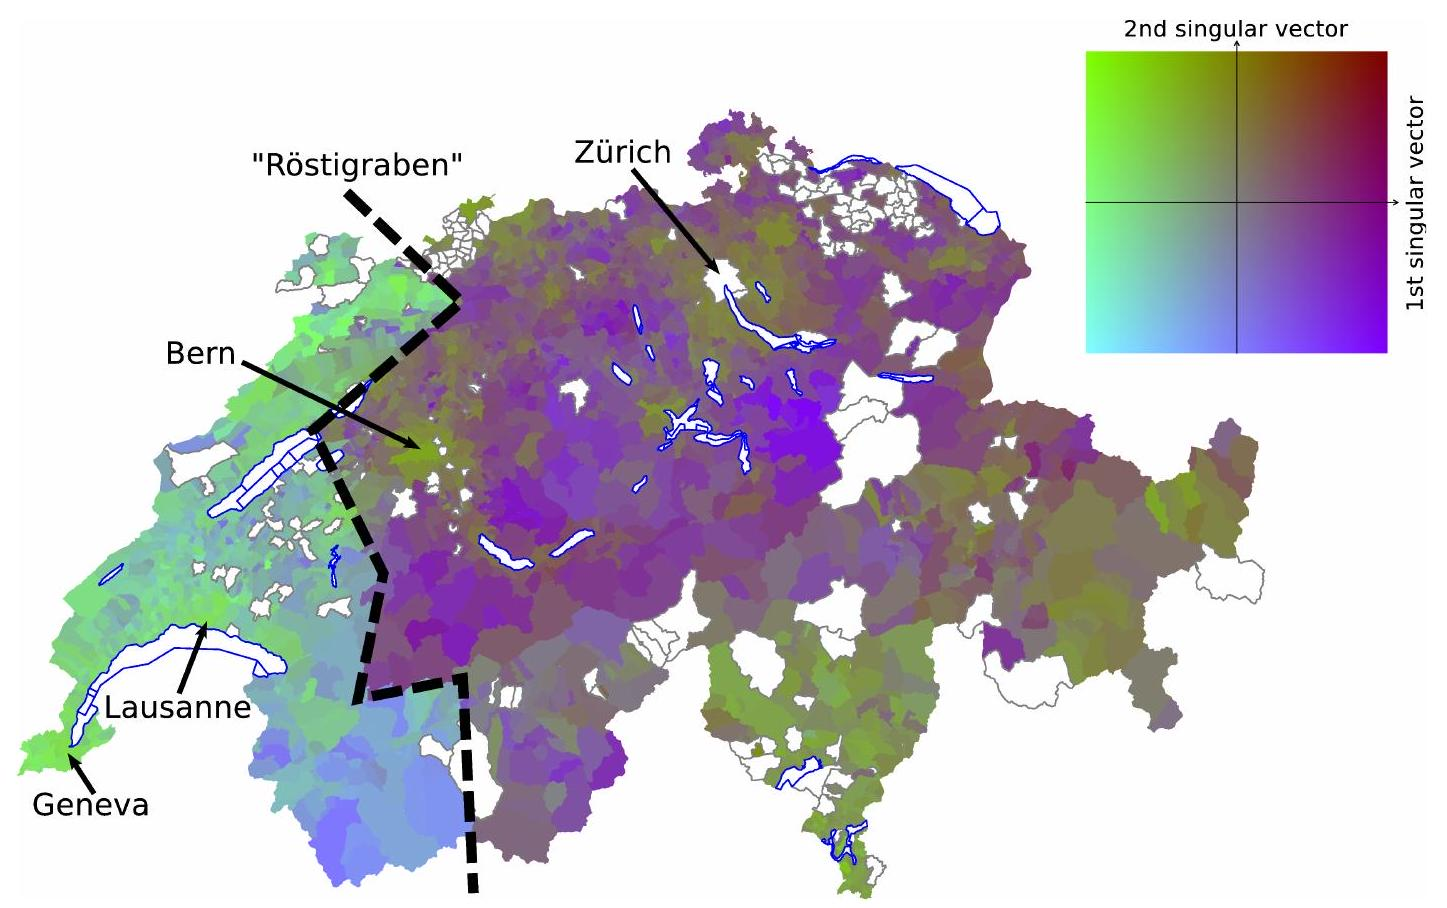
\includegraphics[max width=\textwidth]{2024_01_08_e090cb7d953bac87fc33g-04}
\end{center}

Figure 9: Voting patterns of Swiss municipalities. The color of a municipality is assigned using its location in Figure 8 and the color gradient shown in the upper right corner. Two municipalities with similar colors have similar voting patterns. The Röstigraben, corresponding to the cultural difference between French-speaking municipalities and German-speaking ones, is clearly visible from the difference in voting patterns. Regions shown in white are lakes or municipalities for which some vote results are missing (due to a merging of municipalities, for example). A more detailed map can be found online [2].

\section*{PCA Example 2: Genes mirror geography}
\begin{center}
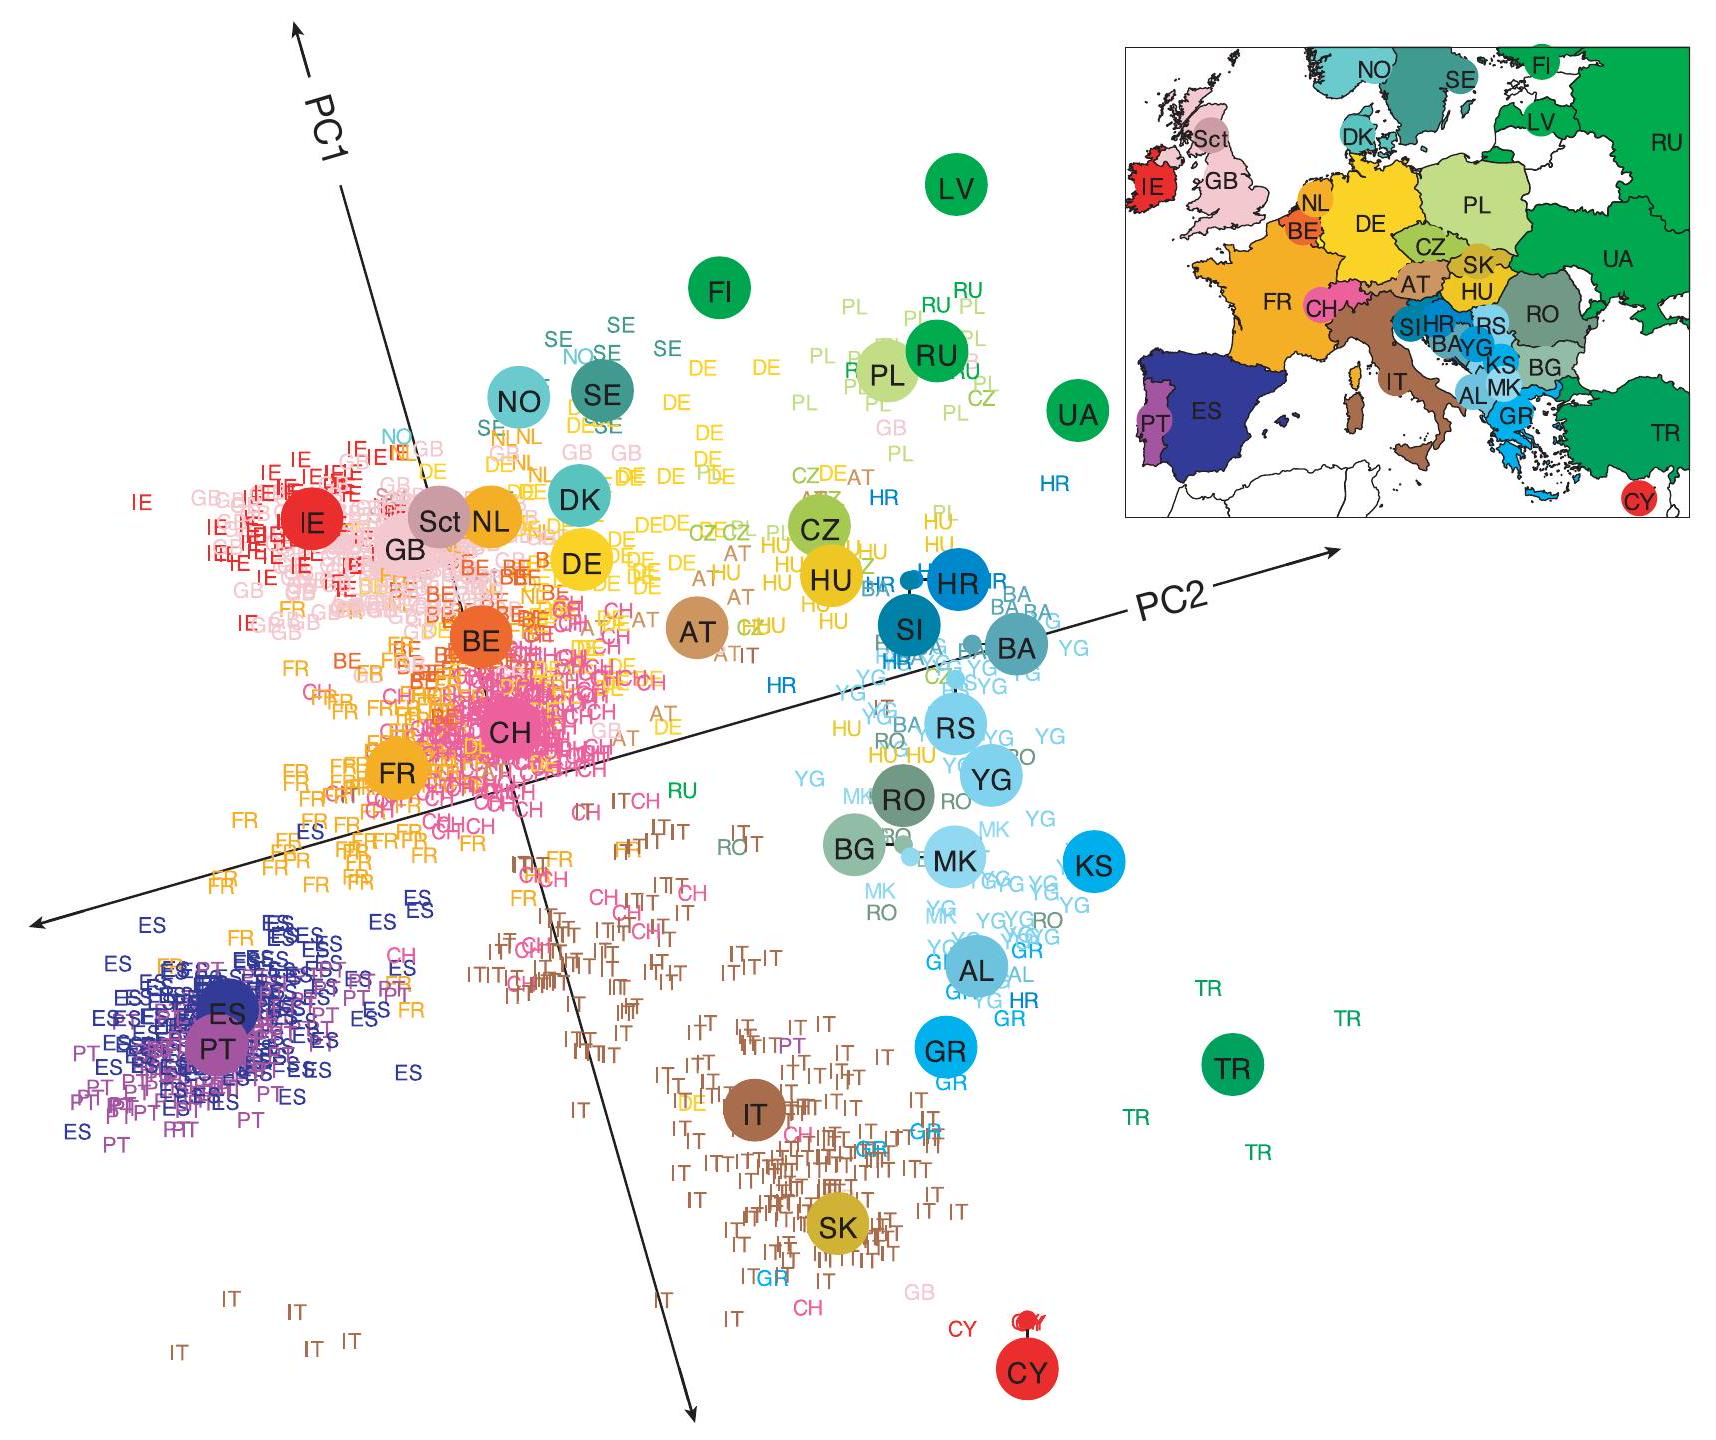
\includegraphics[max width=\textwidth]{2024_01_08_e090cb7d953bac87fc33g-05}
\end{center}

Nature 2008, \href{http://dx.doi.org/10.1038/nature07331}{http://dx.doi.org/10.1038/nature07331}

\section*{Examples for Clustering}
\begin{center}
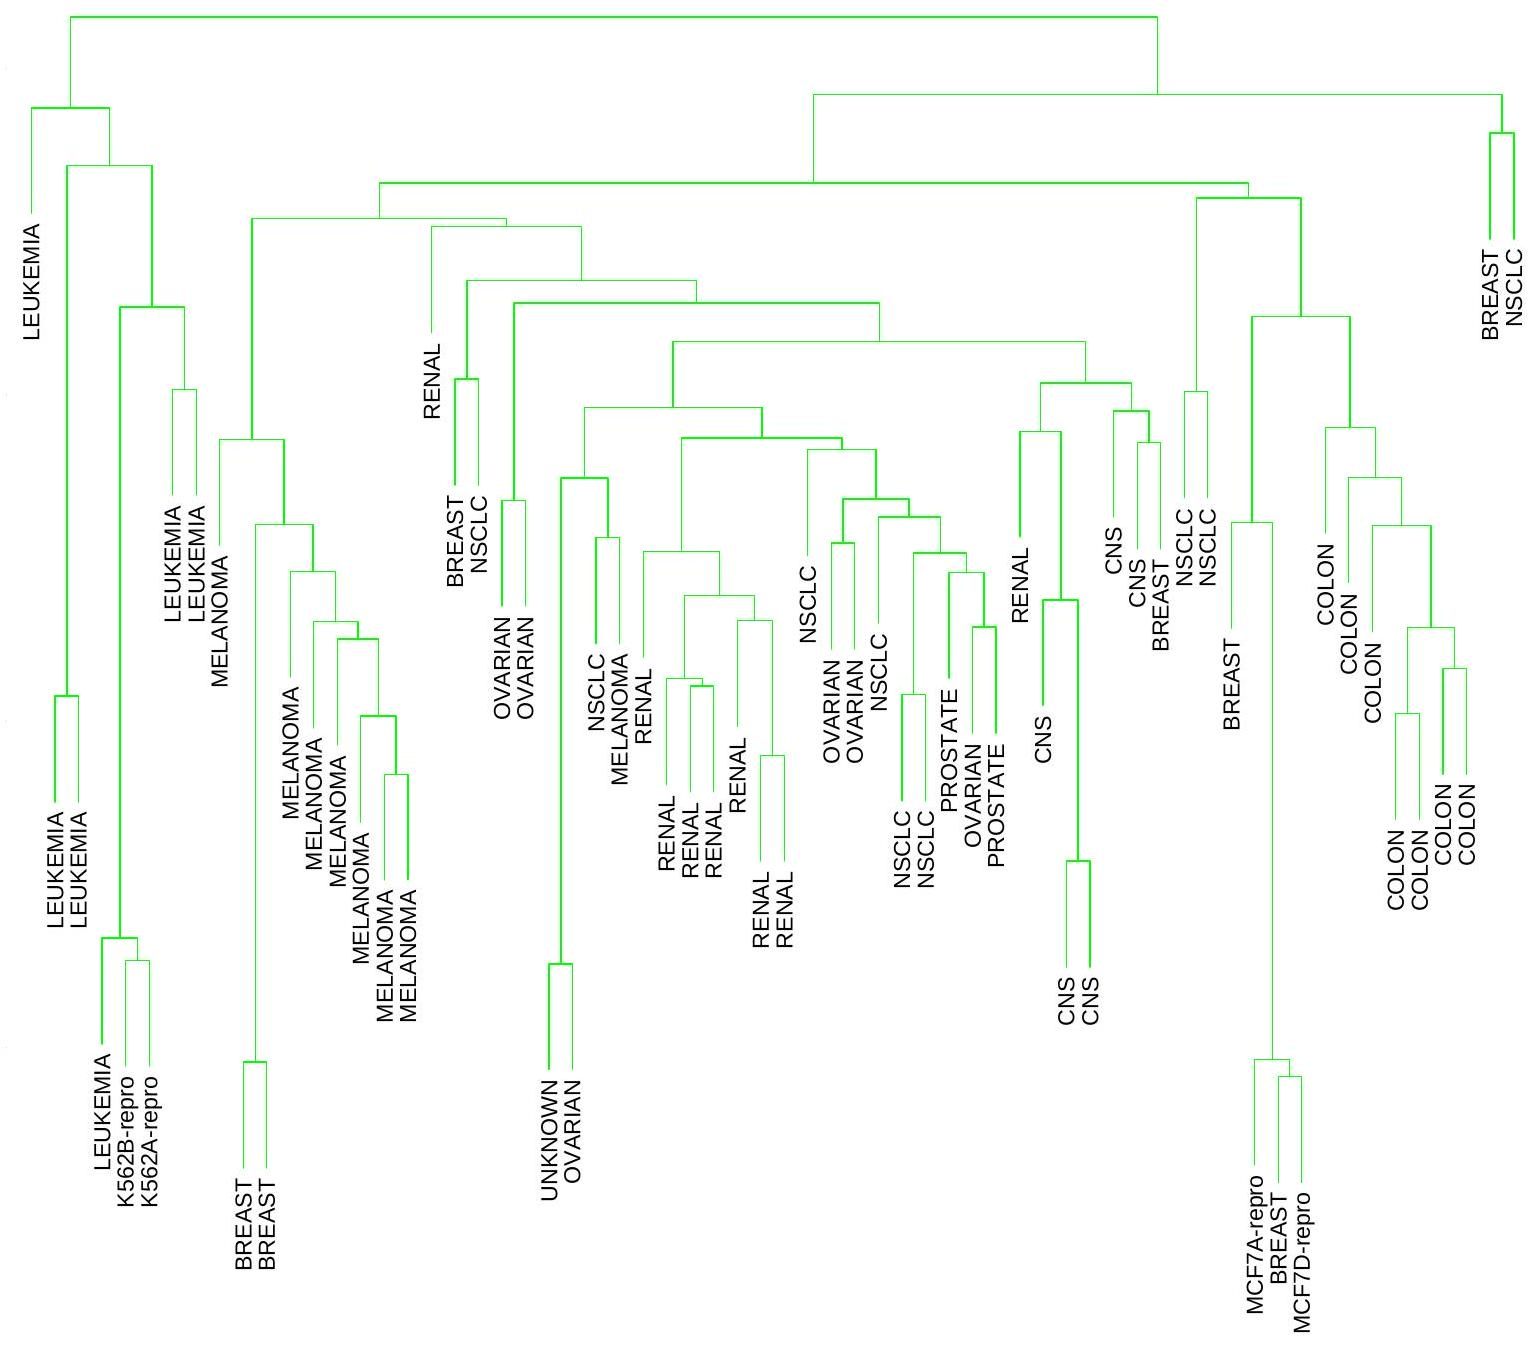
\includegraphics[max width=\textwidth]{2024_01_08_e090cb7d953bac87fc33g-06}
\end{center}

FIGURE 14.12. Dendrogram from agglomerative hierarchical clustering with average linkage to the human tumor microarray data.

\section*{Clustering more than two million biomedical publications (Kevin Boyack et.al. 2011)}
\begin{center}
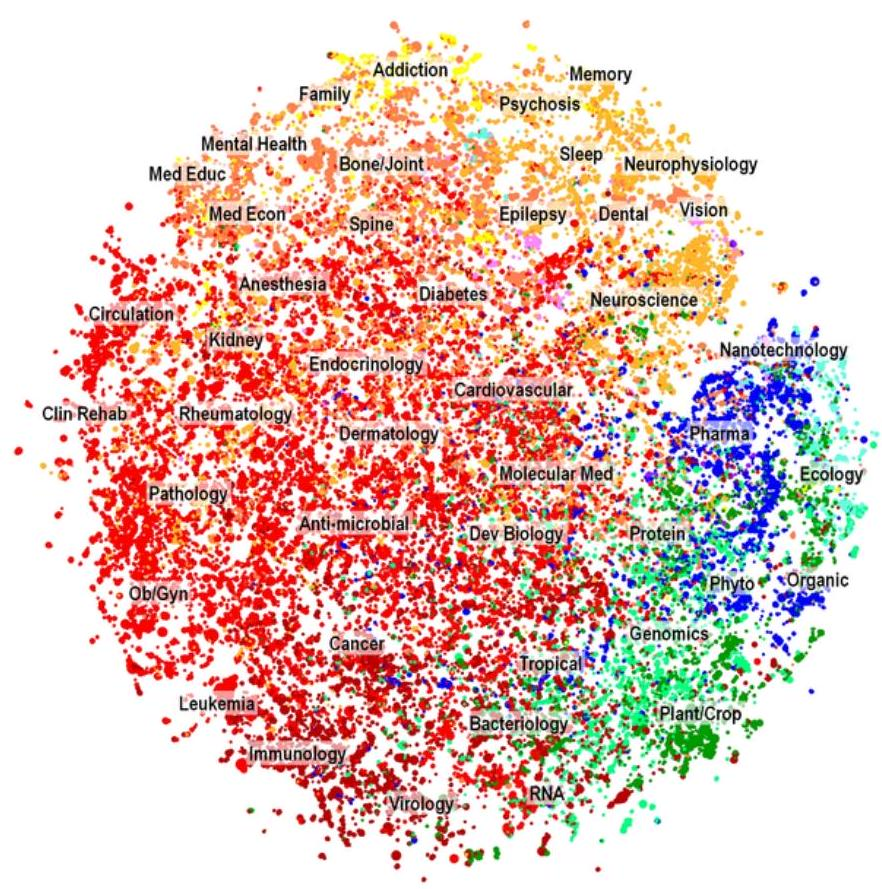
\includegraphics[max width=\textwidth]{2024_01_08_e090cb7d953bac87fc33g-07(1)}
\end{center}

Clustering articles published in Science (Blei \& Lafferty 2007)

\begin{center}
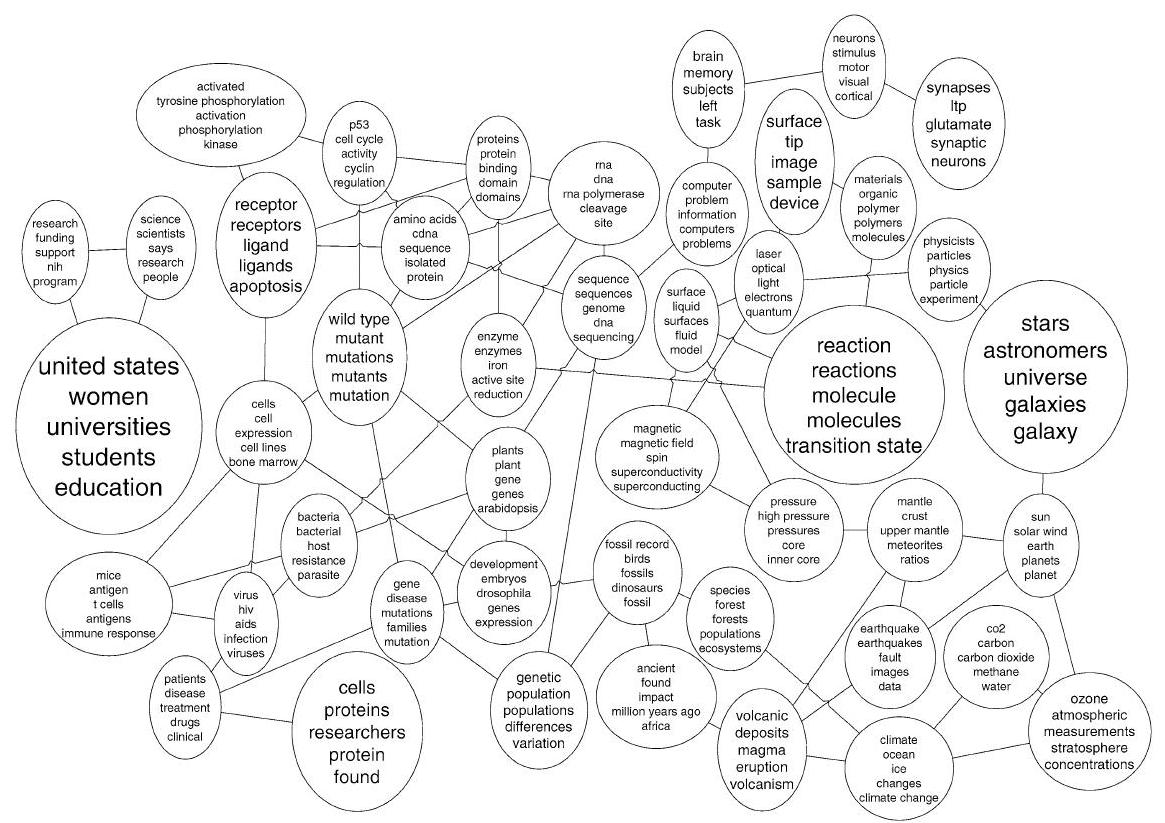
\includegraphics[max width=\textwidth]{2024_01_08_e090cb7d953bac87fc33g-07}
\end{center}

FIG. 2. A portion of the topic graph learned from 16,351 OCR articles from Science (1990-1999). Each topic node is labeled with its five most probable phrases and has font proportional to its popularity in the corpus. (Phrases are found by permutation test.) The full model can be found in \href{http://www.cs.cmu.edu/}{http://www.cs.cmu.edu/} lemur/science/ and on STATLIB.

\section*{Unsupervised Representation Learning \& Generation}
\section*{How does it work?}
Define a unsupervised or self-supervised loss function, for

\begin{itemize}
  \item Compression \& Reconstruction (e.g. Auto-Encoder)
\end{itemize}

\begin{center}
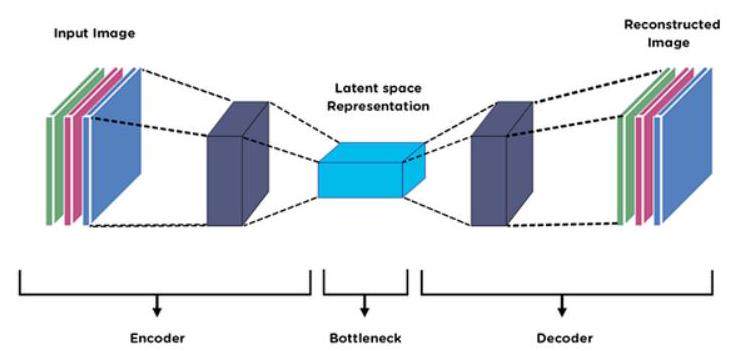
\includegraphics[max width=\textwidth]{2024_01_08_e090cb7d953bac87fc33g-08}
\end{center}

image: Deepak Birla

\begin{itemize}
  \item Consistency \& Contrastive Learning (e.g. Noise-contrastive estimation)
\end{itemize}

\begin{center}
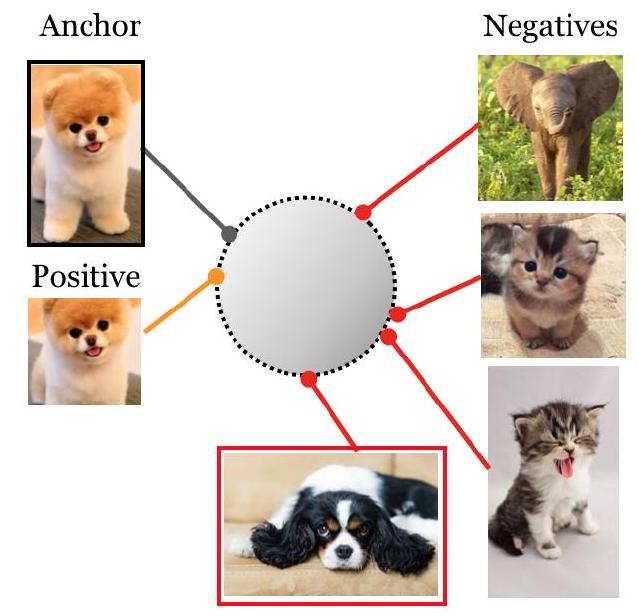
\includegraphics[max width=\textwidth]{2024_01_08_e090cb7d953bac87fc33g-08(1)}
\end{center}

image: \href{http://arxiv.org/pdf/2004.11362}{arxiv.org/pdf/2004.11362}

\begin{itemize}
  \item Generation
\end{itemize}

(e.g. Auto-Encoder, Gaussian Mixture Model)

\section*{Examples:}
$(\mathrm{G}=$ can be used as a generative model $)$

\begin{itemize}
  \item Auto-Encoders (G)
\end{itemize}

Invertible networks, learned compression, normalizing flows

\begin{itemize}
  \item Representation Learning
\end{itemize}

e.g. images, text, time-series, video. Combining unsupervised representation learning (pre-training) with supervised learning

\begin{itemize}
  \item Language Models \& Sequence Models (G)
\end{itemize}

text generation, or sequence continuation, BERT

video, audio \& timeseries (auto-regressive, contrastive, ...)

\begin{itemize}
  \item Generative Adversarial Networks (GAN) (G) see also predictability minimization
\end{itemize}

\begin{center}
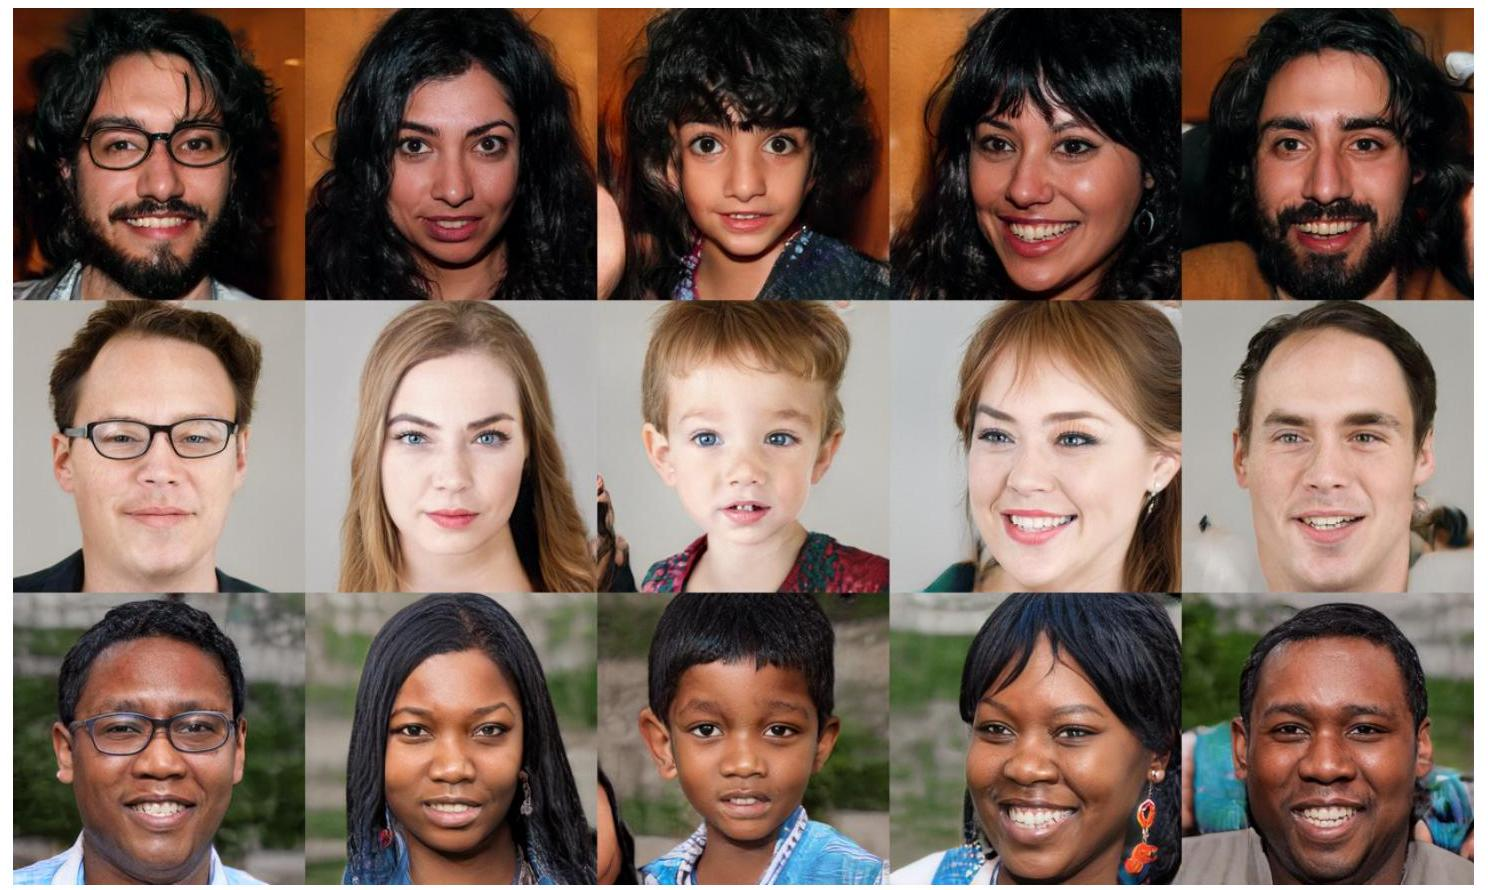
\includegraphics[max width=\textwidth]{2024_01_08_e090cb7d953bac87fc33g-09}
\end{center}

"A Style-Based Generator Architecture for Generative Adversarial Networks", CVPR 2019, \href{https://arxiv.org/abs/1812}{https://arxiv.org/abs/1812}. 04948

\begin{itemize}
  \item Contrastive image-language pretraining (CLIP) learns a joint representation space for images and text using contrastive learning

  \item Diffusion models (G) new state-of-the-art in image generation; these models can be adapted to generate images from text prompts (e.g., DALL-E 2, Stable Diffusion, Midjourney)

\end{itemize}

\begin{center}
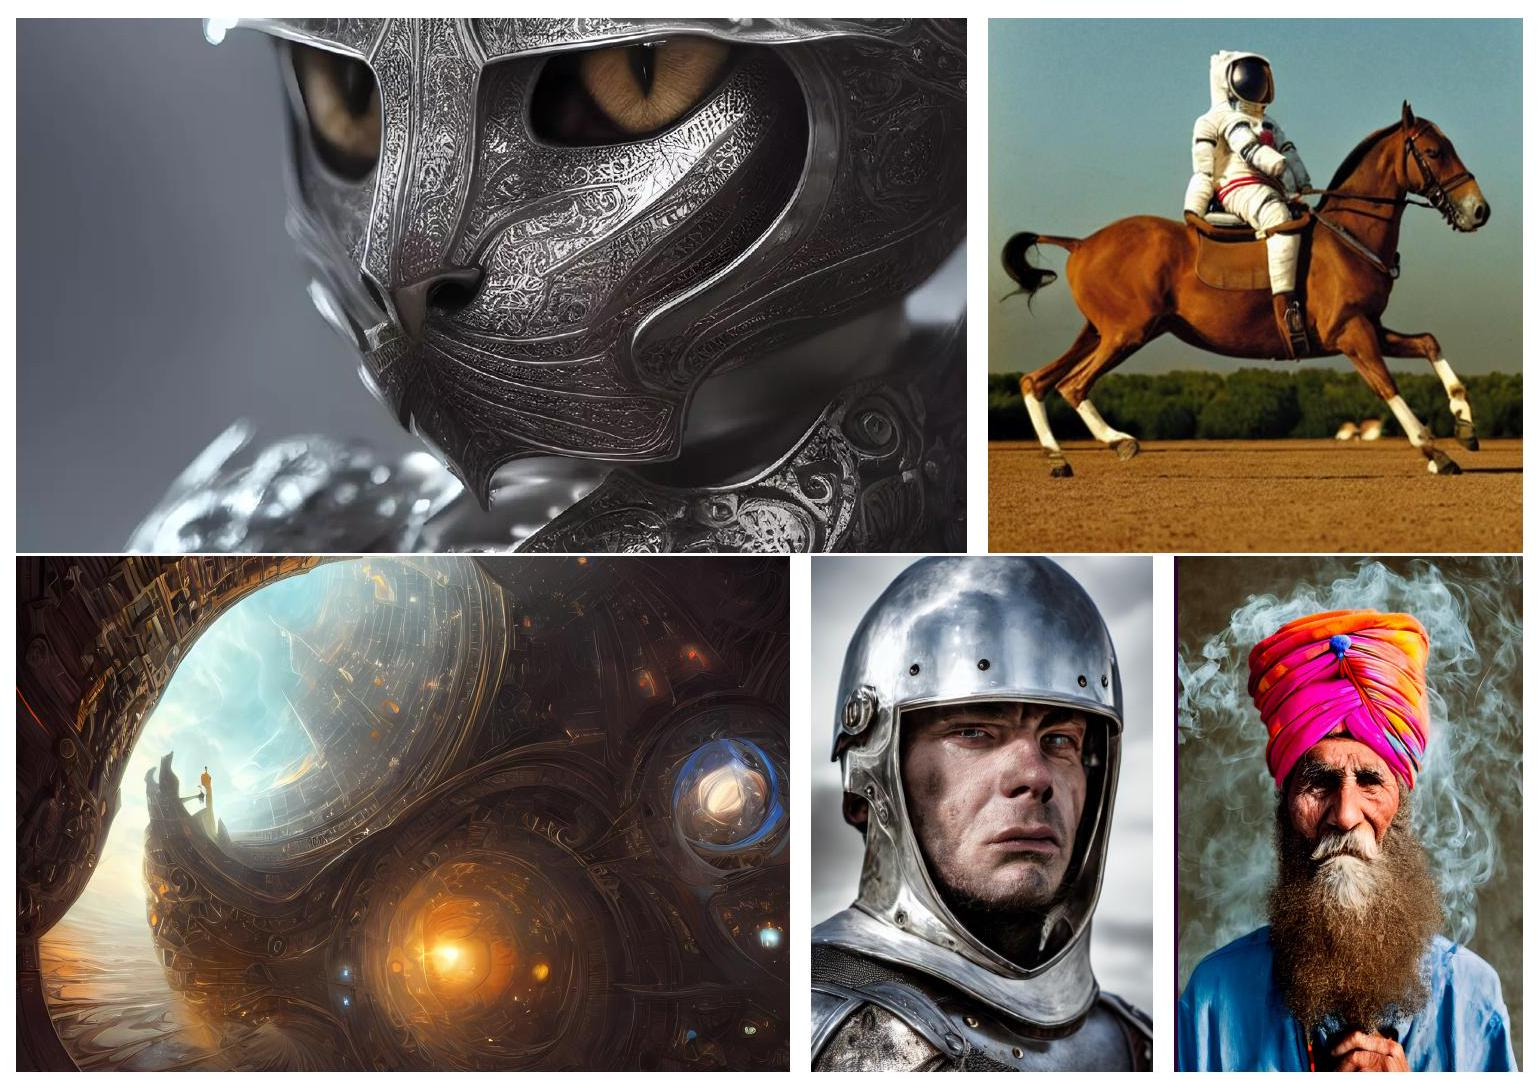
\includegraphics[max width=\textwidth]{2024_01_08_e090cb7d953bac87fc33g-10}
\end{center}

Source: Stable Diffusion model \href{https://stability.ai/blog/stable-diffusion-public-release}{https://stability.ai/blog/stable-diffusion-public-release}


\end{document}